\documentclass[aspectratio=1610]{beamer}

\usetheme{unnslides}
\usefonttheme{professionalfonts}

\usepackage[T2A]{fontenc}
\usepackage[utf8]{inputenc}
\inputencoding{utf8}
\usepackage{listings}
\usepackage{graphicx}
\usepackage{caption}
\usepackage{cmbright}
\usepackage{fontspec}
\usepackage{unicode-math}
\usepackage{amsfonts}
\usepackage{subfig}
\usepackage{tikz}
\usepackage{amsthm}

\captionsetup[subfigure]{labelformat=empty}
\captionsetup[figure]{labelformat=empty}

\setmainfont{CMU Sans Serif}
\setromanfont{CMU Sans Serif}
\setsansfont{CMU Sans Serif}

\setlength{\tabcolsep}{1pt}

\usepackage{polyglossia}
\setmainlanguage{russian}
%\setbeamertemplate{itemize item}{\color{black}$\blacktriangleright$}

\DeclareMathOperator*{\argmax}{arg\,max}
\DeclareMathOperator*{\argmin}{arg\,min}
\DeclareMathOperator{\sign}{sign}
\DeclareMathOperator{\re}{Re}


\graphicspath{ {../images/}{img/} }

%set pages numeration
\newcommand\numbered{\setbeamertemplate{footline}{%
  \vspace{-10em}
   \raisebox{5pt}{\makebox[\paperwidth]{%
     \hfill\makebox[10pt]{%
       \usebeamerfont{footline}\usebeamercolor[fg]{footline}
       \insertframenumber}}}}}
\newcommand\unnumbered{\setbeamertemplate{footline}{}}

\title{Разработка и исследование способов распределения ресурсов в
параллельных алгоритмах глобальной оптимизации}
\author{\textbf{Соврасов~В.В}, научный руководитель: Баркалов~К.А.}
\institute{ННГУ им. Н.И.~Лобачевского}
\date{}

\begin{document}
\numbered
{
\unnumbered
\begin{frame}[noframenumbering,plain]
\titlepage
\end{frame}
}

\begin{frame}
  \frametitle{Структура работы}
  \begin{enumerate}
    \setlength{\itemindent}{.1in}
    \item[Глава 1.] Методы редукции размерности, их сравнение
    \item[Глава 2.] Сравнение актуальных методов глобальной оптимизации
    \item[Глава 3.] Метод для решения множества задач с ограничениями
  \end{enumerate}
\end{frame}


\begin{frame}
  \frametitle{Постановка задачи глобальной оптимизации}
  \begin{columns}
    \begin{column}{0.5\textwidth}
      \begin{displaymath}
        \begin{array}{cr}\\
          \varphi(y^*)=\min\{\varphi(y):y\in G\},\:G=D \cap \{y:\\
           g_j(y)\leqslant 0, 1\leqslant j\leqslant m\},
        \end{array}
      \end{displaymath}
      где \(D\) -- прямоугольник в \(\mathbb{R}^N\),
      \(\varphi(y),\:g_j(y)\) -- многоэкстремальные функции, удовлетворяющие условию Липшица в \(D\):
      \begin{displaymath}
          |f(y_1)-f(y_2)|\leqslant L\Vert y_1-y_2\Vert,y_1,y_2\in D,
      \end{displaymath}
      где \(L>0\) -- константа Липшица, а \(||\cdot||\) обозначает \(l_2\)-норму в \(\mathbb{R}^N\).
    \end{column}
    \begin{column}{0.5\textwidth}
      \centerline{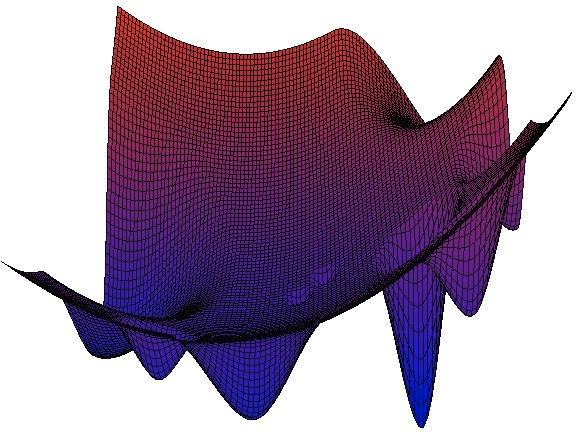
\includegraphics[width=0.9\textwidth]{img/gkls.png}}
    \end{column}
  \end{columns}
\end{frame}

\begin{frame}
  \frametitle{Постановка задачи глобальной оптимизации}
  Рассмотрим множество из \(q\) глобальной оптимизации с ограничениями-неравенствами:
  \begin{equation}
    \label{eq:many_problems}
    \min\left\{\varphi_1(y), y\in G_1 \right\}, \min\left\{\varphi_2(y), y\in G_2\right\},...,
  \min\left\{\varphi_q(y), y\in G_q\right\}.
  \end{equation}
  Будем считать, что метод оптимально распоряжается ресурсами, если при его остановке на некоторой итерации
  решение всех задач получено с одинаковой точностью. Такого свойства можно добиться, потребовав
  от метода равномерной сходимости на всём множестве задач:
  \begin{equation}
    \exists \varepsilon > 0: \forall s>1, \forall i,j\in\{1,\dots,q\}\;
      \frac{\Vert \overline{y_i}^*(s) - y_i^*\Vert_\infty}{\Vert \overline{y_j}^*(s) - y_j^*\Vert_	\infty} \leqslant \varepsilon,
  \end{equation}
  где \(s\) это количество итераций метода оптимизации, \(\tilde{y_i}(s)^*\) это приближение к решению, полученное методом в задаче \(i\)
  из множества (\ref{eq:many_problems}) на итерации \(s\).

\end{frame}

\begin{frame}
  \frametitle{Решение множества задач}
  Упомянутые множества задач могут возникнуть, например, в следующих случаях:
  \begin{itemize}
    \item наличие у непрерывной задачи дискретного параметра, который принимает ограниченный диапазон значений;
    \item набор задач получен при скаляризации задачи многокритериальной оптимизации.
  \end{itemize}
\textbf{Возможные подходы}:
  \begin{itemize}
    \item решать каждую задачу независимо;
    \item разработать метод оптимизации, решающий все задачи "одновременно", в каждый момент времени приоритизируя одну из них.
  \end{itemize}
\end{frame}

\begin{frame}
  \frametitle{Редукция размерности с помощью развёрток}
  \begin{center}
  Кривая типа Пеано \(y(x)\) позволяет снизить размерность исходной задачи оптимизации:
  \begin{gather}
    D_e=\lbrace y\in \mathbb{R}^N:-2^{-1}\leqslant y_i\leqslant 2^{-1},1\leqslant i\leqslant N\rbrace=\{y(x):0\leqslant x\leqslant 1\} \nonumber \\
    \min\{\varphi(y): y\in D\}=\min\{\varphi(y(x)): x\in [0,1]\} \nonumber
  \end{gather}
  \(y(x)\) является негладкой непрерывной функцией, отображающей отрезок \([0,1]\) на гиперкуб \(D_e\).
  \begin{figure}[ht]
    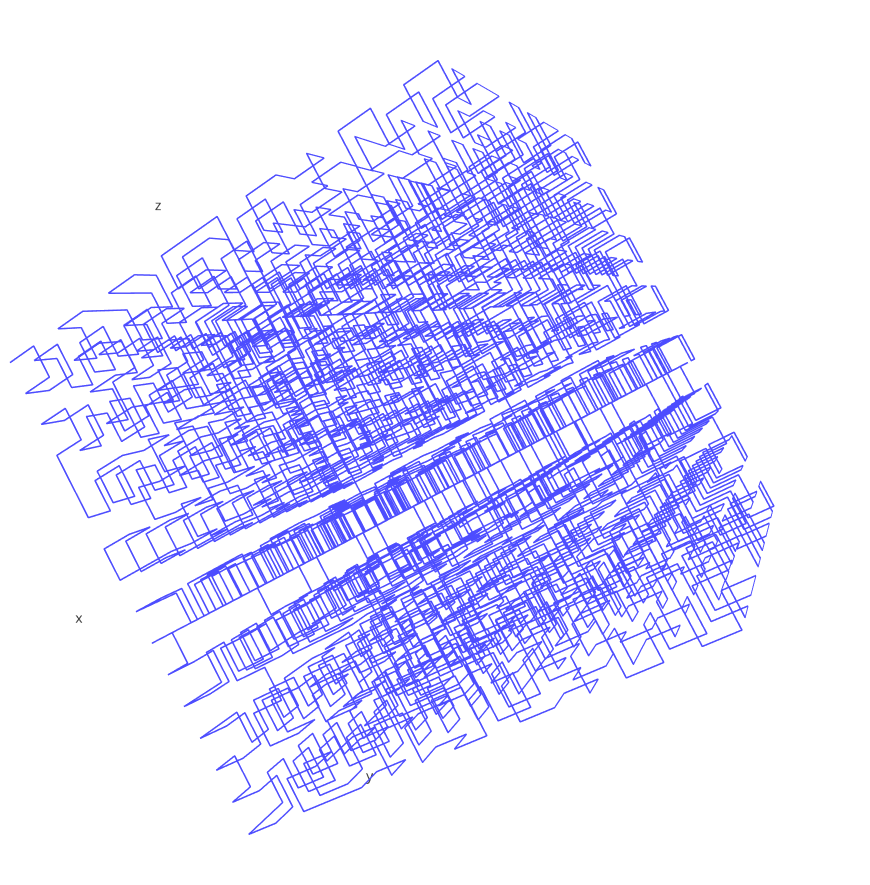
\includegraphics[width=.3\textwidth]{peano3d.png}
    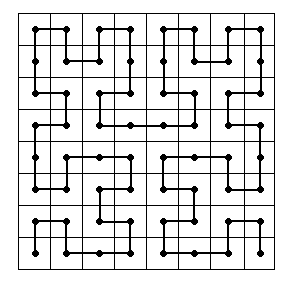
\includegraphics[width=.3\textwidth]{peano2d.png}
  \end{figure}
\end{center}
\end{frame}

\begin{frame}
  \frametitle{Свойства задачи после редукции}
  После применения развёртки, \(\varphi(y(x))\) удовлетворяет условию Гёльдера:
  \begin{displaymath}
    |\varphi(y(x_1))-\varphi(y(x_2))|\leq H{|x_1-x_2|}^{\frac{1}{N}}, x_1,x_2\in[0,1],
  \end{displaymath}
  \(\varphi(y(x))\) является негладкой функцией с множеством локальных и глобальных экстремумов \textbf{global}, даже если \(\varphi(y)\) унимодальна.
  Появление дополнительных экстремумов связано с потерей информации о \(N\)-мерных окрестностях точек после применения отображения в одномерное пространство.

  \begin{figure}[ht]
    \begin{center}
    \vspace*{-0.5cm}
    \subfloat{\raisebox{.02\textheight}{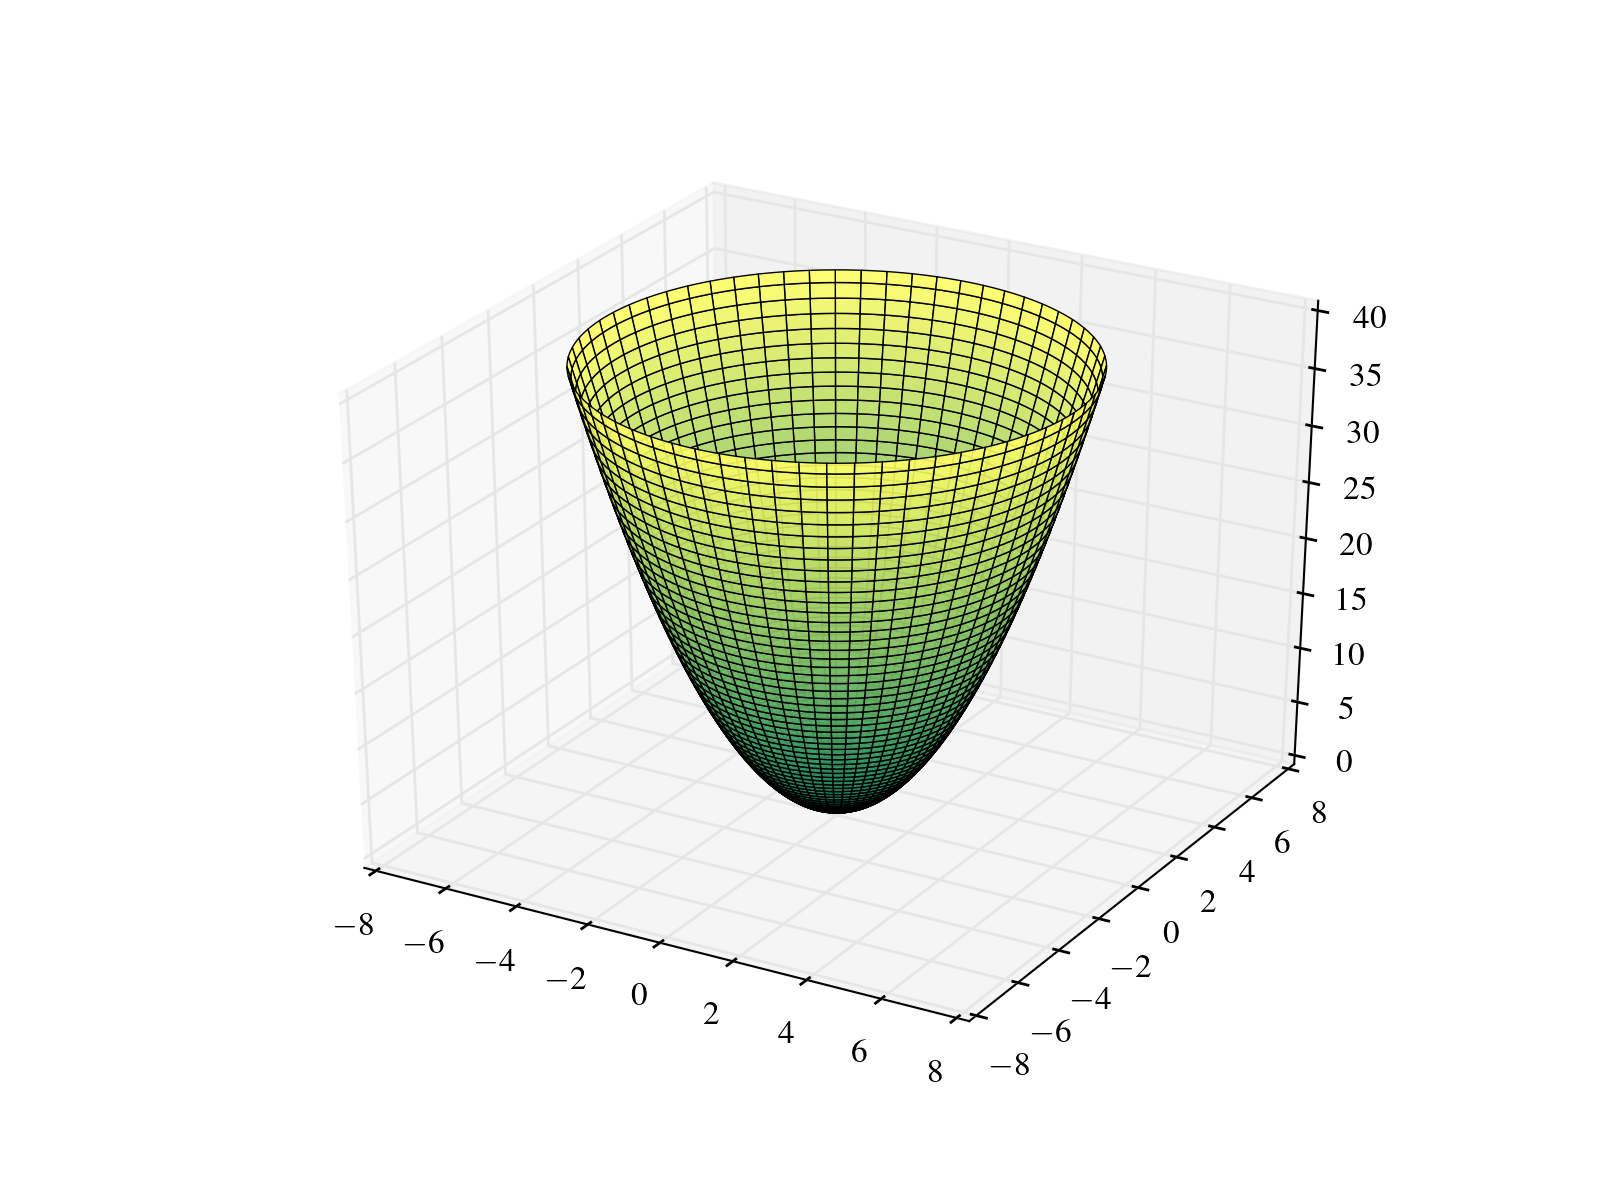
\includegraphics[width=.4\textwidth]{parabaloid.png}}}
    \subfloat{\raisebox{.2\textheight}{
\includegraphics[width=.05\textwidth]{arrow.jpg}}}
    \subfloat{{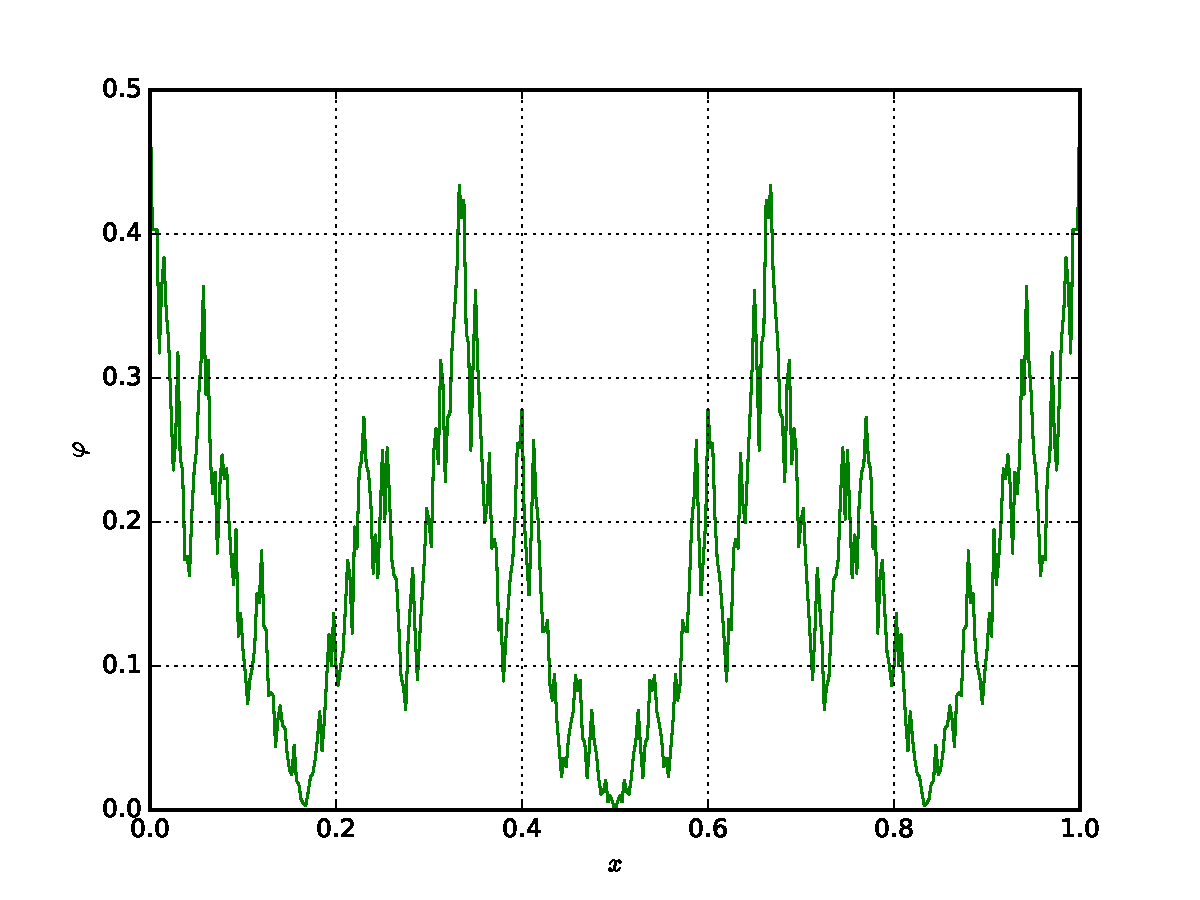
\includegraphics[width=.45\textwidth]{map_paraboloid.pdf}}}
  \end{center}
  \end{figure}
\end{frame}

\begin{frame}
  \frametitle{Схема одномерного характеристического алгоритма оптимизации}
  Метод генерирует последовательность точек \(\{x_k:x_k\in[a,b]\}\), выполняя следующие шаги:
  \begin{enumerate}
    \setlength{\itemindent}{.1in}
    \item[Шаг 1.] Отсортировать поисковую информацию (одномерные точки) в порядке возрастания координаты.
    \item[Шаг 2.] Для каждого интервала \((x_{i-1}, x_i)\) вычислить величину \(R(i)\), называемую характеристика.
    \item[Шаг 3.] Выбрать интервал с наибольшей характеристикой, \((x_{t-1}, x_{t})\), и
    произвести испытание (вычислить ограничения и целевую функцию) в точке \(x^{k+1}\), выбранной в соответствии с решающим правилом \(d\):
    \begin{displaymath}
      x^{k+1}=d(t)\in (x_{t-1}, x_{t})
    \end{displaymath}
    \item[Шаг 4.] Если верно \(x_{t}-x_{t-1}<\varepsilon\), остановить работу метода.
  \end{enumerate}
  \textit{\footnotesize	{Описание характеристического метода AGS приведено в Strongin R.G., Sergeyev Ya.D.: Global optimization with non-convex constraints. Sequential and parallel algorithms (2000), Chapter 7}}
\end{frame}

\begin{frame}
  \frametitle{Неинъективная развёртка}
    Одним из подходов к восстановлению потерянной информации является вычисление всех прообразов точки \(y\in\mathbb{R}^N\) 
    и их учёт в методе оптимизации\footnote{Р.Г. Стронгин. Численные методы в многоэкстремальных задачах, 1978}.
    Это позволяет снизить влияние эффекта расщепления локальных экстремумов.
    Каждая \(N\)-мерная точка может иметь до \(2^N\) прообразов, поэтому
    для большого значения \(N\) вычисление и учёт их всех становится трудоёмким.
      \begin{figure}[ht]
        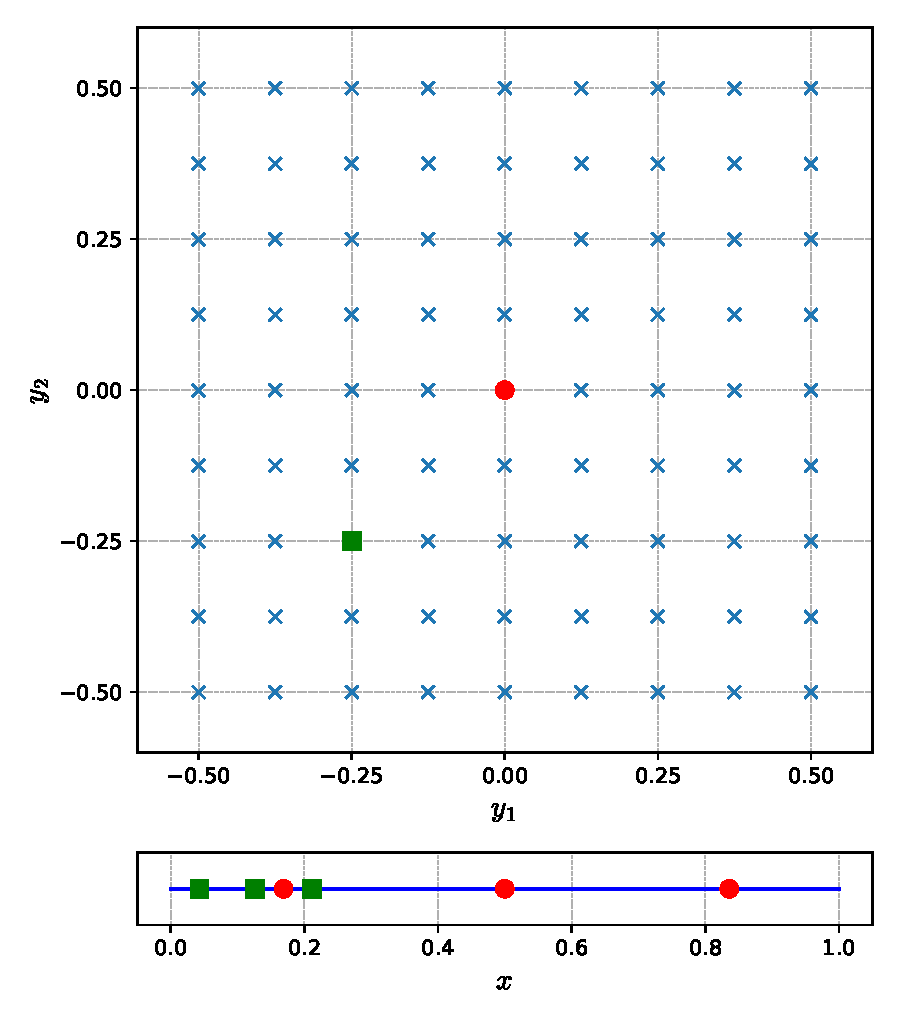
\includegraphics[width=.25\textwidth]{evolvents/noninjective.pdf}
      \end{figure}
\end{frame}

\begin{frame}
  \frametitle{Сдвиговые и вращаемые развёртки}
  Получить фиксированное количество одномерных прообразов можно, например, используя заранее выбранный набор инъективных развёрток.
  Подобных набор может быть получен путём сдвига или вращения огигинальной развёртки. 
  Набор сдвиговых развёрток\footnote{Strongin, R.G. Algorithms for multi-extremal mathematical programming problems employing the set of joint space-filling curves, Journal of Global Optimization 2(4), 357--378, 1992}
  обладает свойством генерировать как минимум одну пару близких прообразов, для двух близких многомерных точек.
  Для вращаемых развёток подобного утверждения доказано не было, но на практике их использование также приносит ускорение сходимости.
  \begin{figure}[ht]
    \subfloat{\raisebox{.0\textheight}{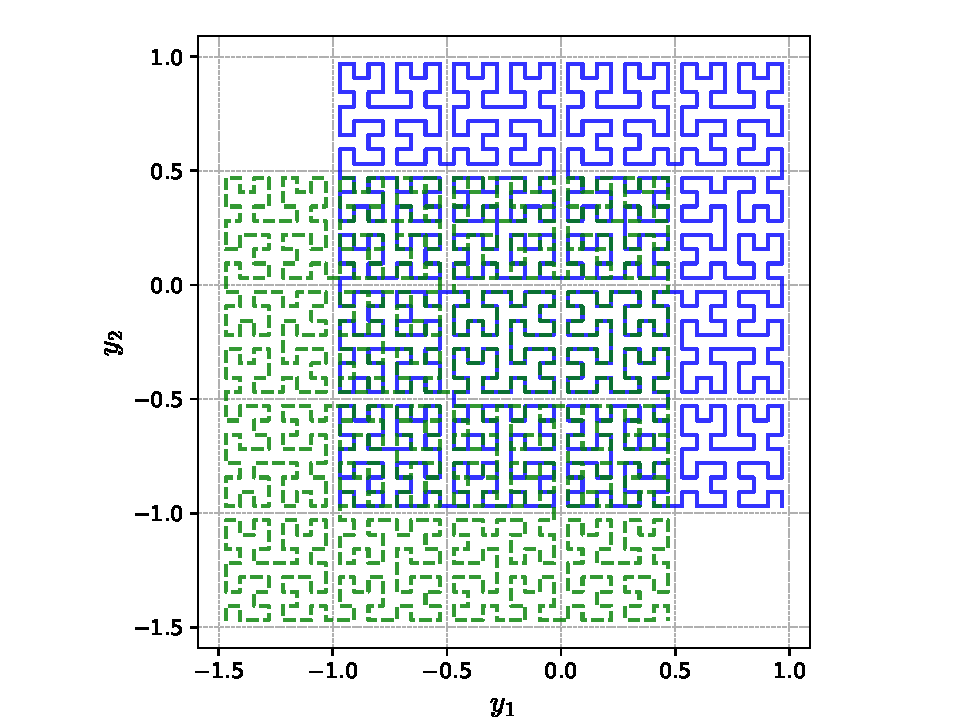
\includegraphics[width=.35\textwidth]{evolvents/shifted.pdf} }}
    \subfloat{{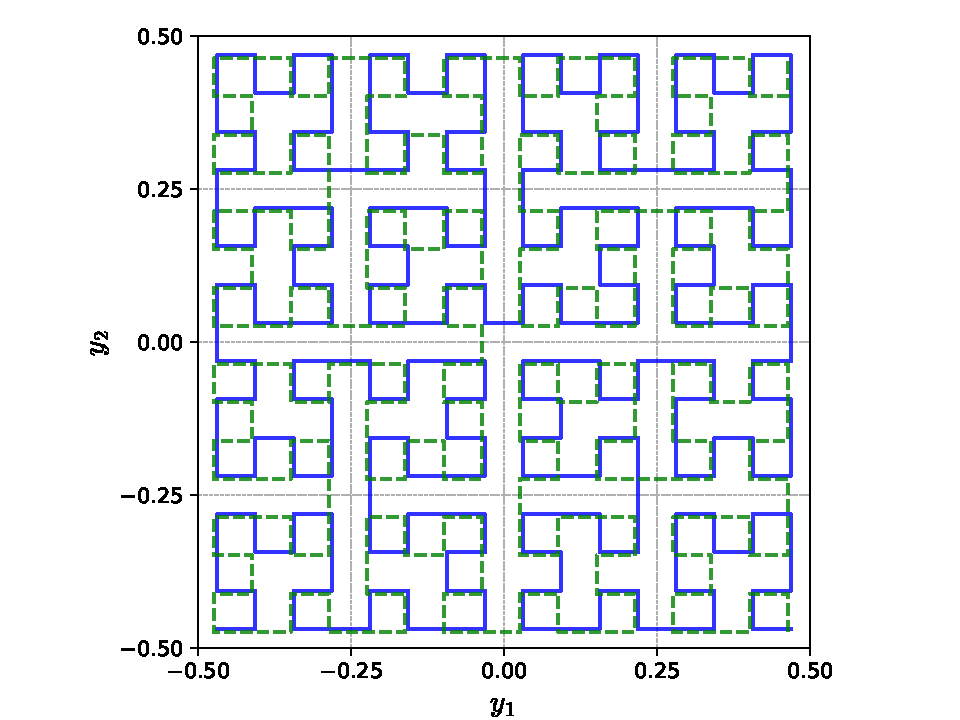
\includegraphics[width=.35\textwidth]{evolvents/rotated.pdf} }}
  \end{figure}
\end{frame}

\begin{frame}
  \frametitle{Гладкая развёртка}
  Поскольку гладкие функции ведут себя более предсказуемо, гладкая аппроксимация кривой Пеано \(y(x)\)
  может ускорить сходимость процесса оптимизации \footnote{Goryachih, A. A class of smooth modification of space-filling curves for global optimization problems, NET 2016}.
  \begin{figure}[ht]
    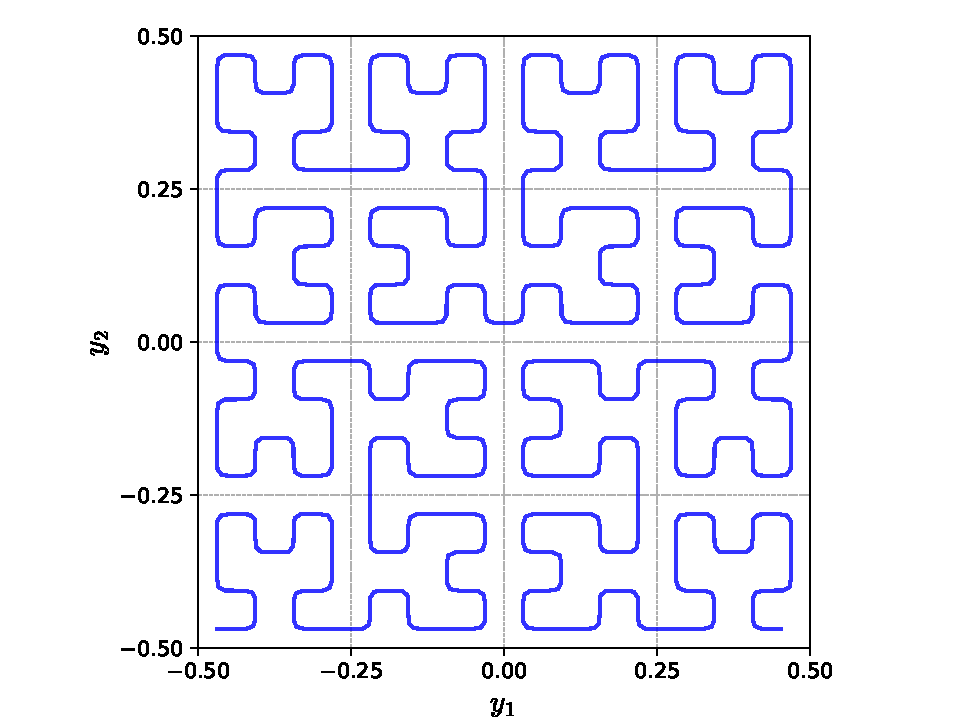
\includegraphics[width=0.45\textwidth]{evolvents/smooth.pdf}
  \end{figure}
\end{frame}


\begin{frame}
  \frametitle{Класс тестовых задач}
  \begin{columns}
    \begin{column}{0.5\textwidth}
      Генератор GKLS (Gaviano, M. et al, 2003):
      \begin{displaymath}
        \begin{matrix}
          f(x)=
          \left\{
          \begin{matrix}
          C_i(x), x \in S_i, i\in 2,\dots ,m \\
          \Vert x-T \Vert^2 + t, x\not\in S_2,\dots,S_m
          \end{matrix} \right.
        \end{matrix}
      \end{displaymath}

      \begin{itemize}
        \item варьируемое число локальных минимумов;
        \item варьируемый размер области притяжения глобального минимума;
        \item размерность функции также задаётся.
      \end{itemize}
    \end{column}
    \begin{column}{0.5\textwidth}
      \centerline{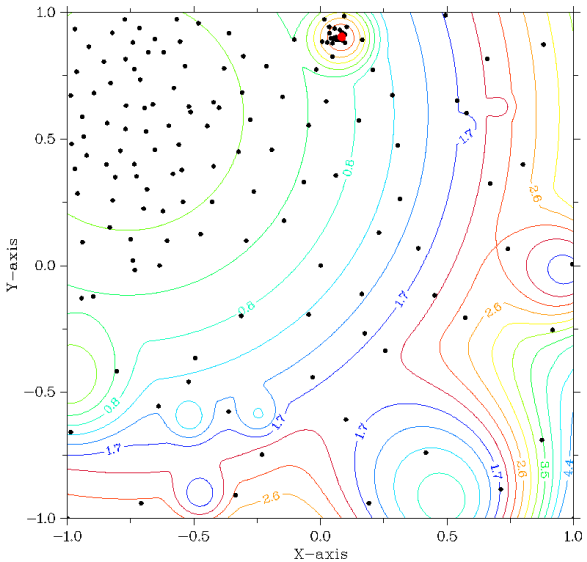
\includegraphics[width=0.9\textwidth]{gkls_color.png}}
    \end{column}
  \end{columns}
  Также был использован один набор из 100 фиксированных многоэкстремальных функций (с 10-30 локальными минимумами). Обозначим его \(F_{GR}\).
\end{frame}


\begin{frame}
  \frametitle{Сравнение развёрток}
  \begin{figure}[ht]
    \hspace*{-0.9cm}
    \subfloat[Minimal \(r\)]{{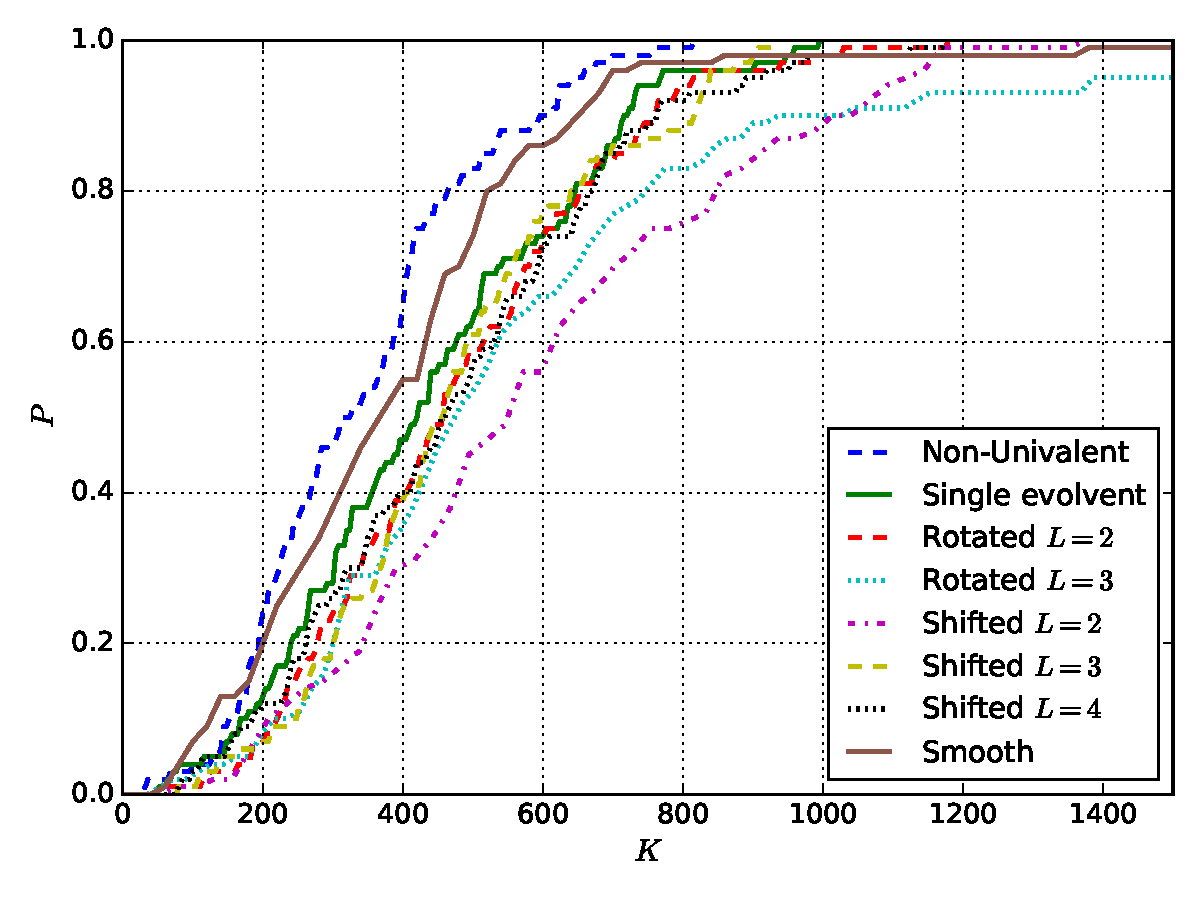
\includegraphics[width=.55\textwidth]{evolvents/gklsS2d_opt_pt_op.pdf} }}
    \subfloat[\(r=5.0\)]{{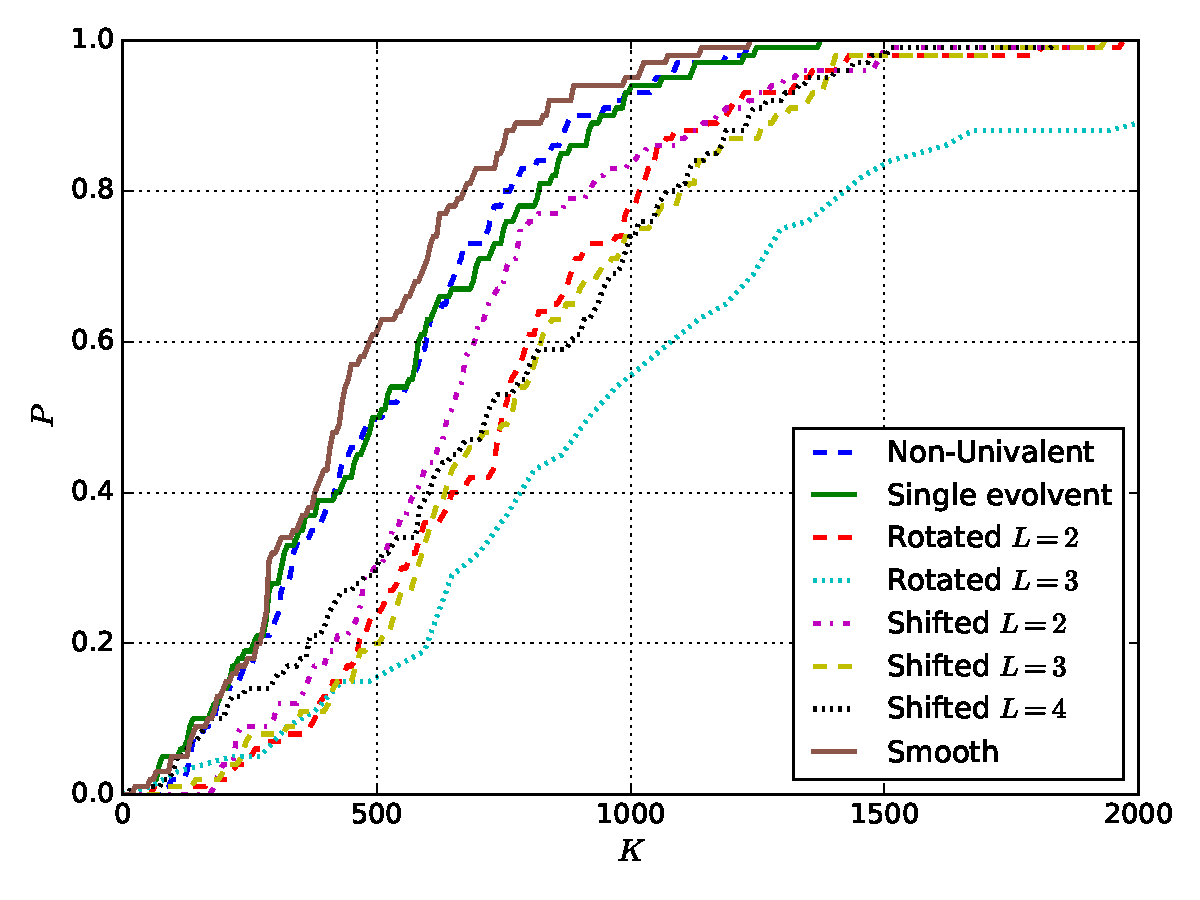
\includegraphics[width=.55\textwidth]{evolvents/gklsS2d_same_r_opt_pt_op.pdf} }} \hspace*{4cm}
    \caption{Операционные характеристики на классе задач GKLS 2d Simple}
  \end{figure}
\end{frame}


\begin{frame}
  \frametitle{Сравнение развёрток}
  \begin{figure}[ht]
    \hspace*{-0.9cm}
    \subfloat[Minimal \(r\)]{{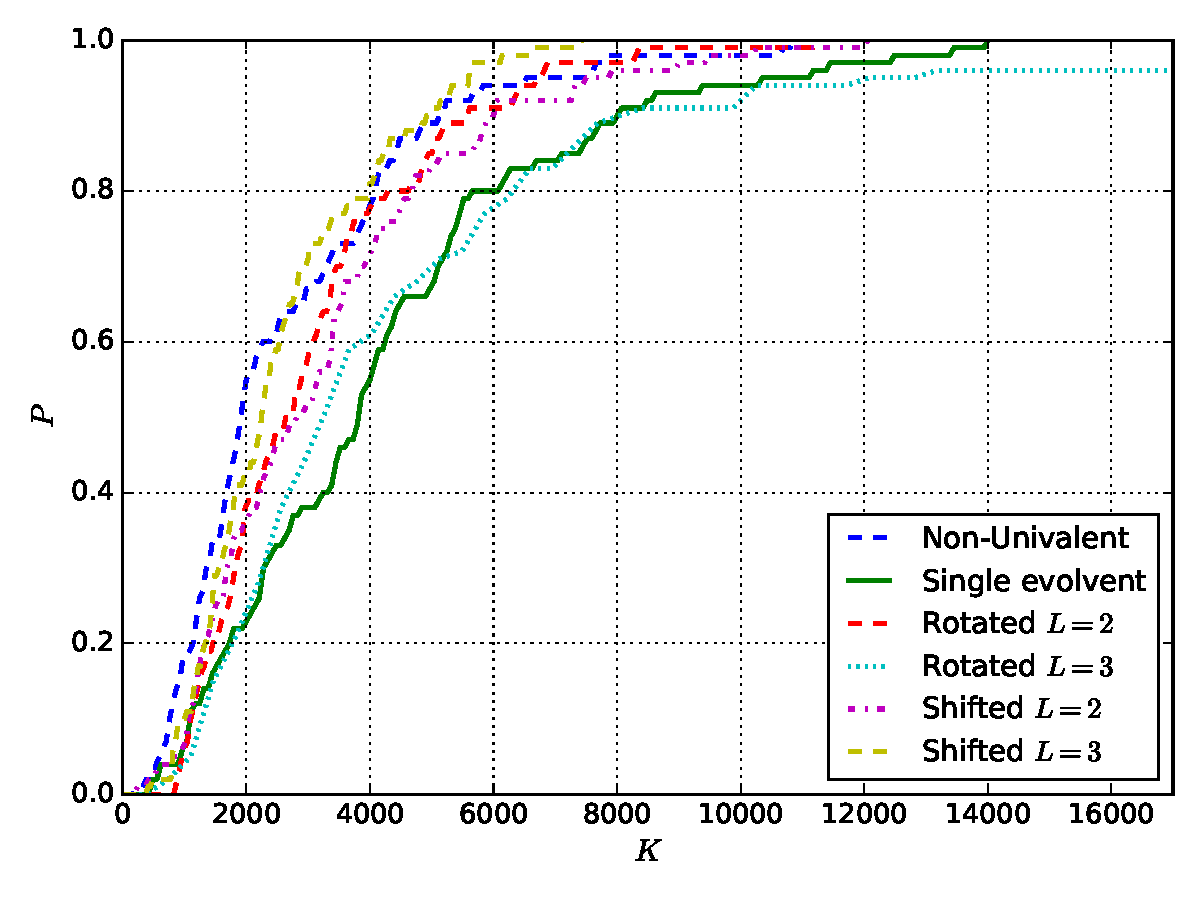
\includegraphics[width=.55\textwidth]{evolvents/gklsS3d_opt_pt_op.pdf} }}
    \subfloat[\(r=4.5\)]{{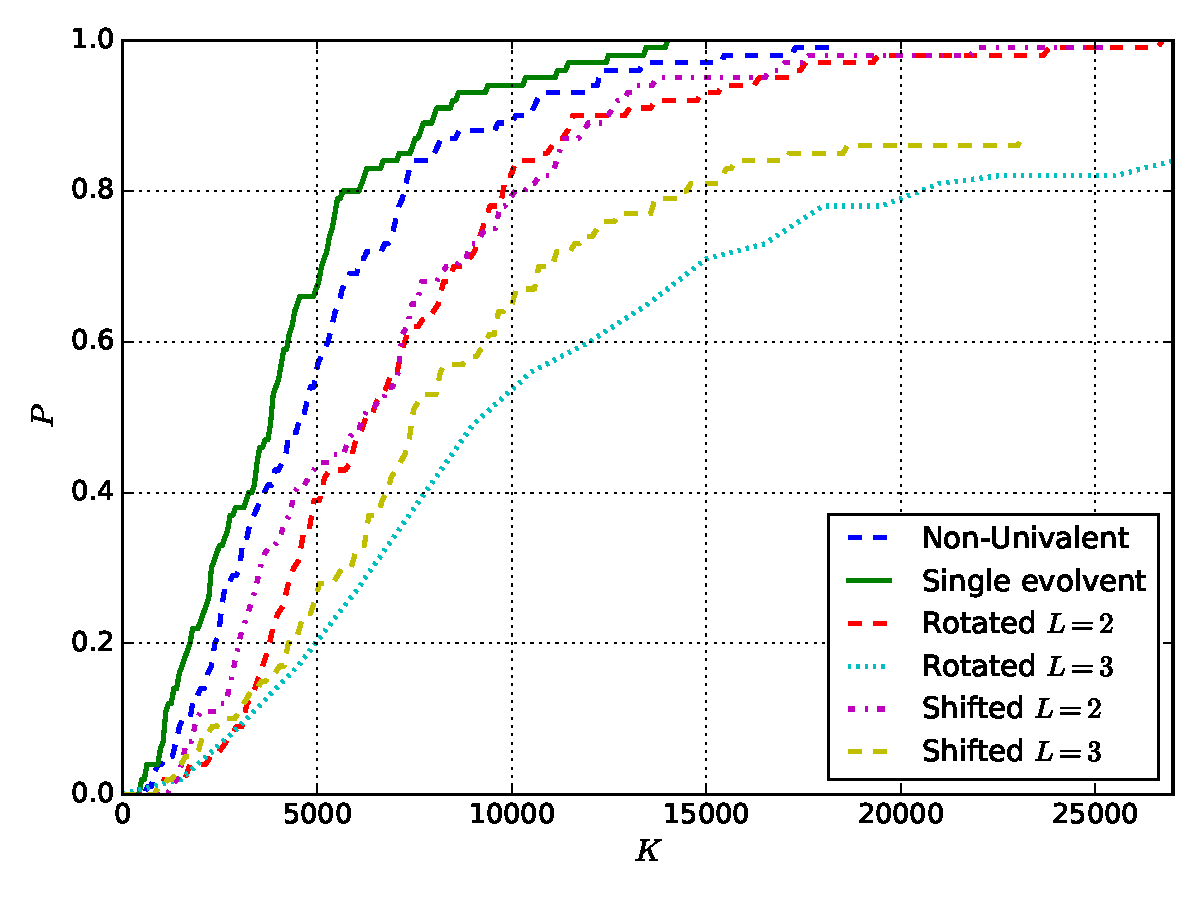
\includegraphics[width=.55\textwidth]{evolvents/gklsS3d_same_r_opt_pt_op.pdf} }}
    \caption{Операционные характеристики на классе задач GKLS 3d Simple}
  \end{figure}
\end{frame}


\begin{frame}
  \frametitle{Сравнение методов глобальной оптимизации}
  Рассмотрим следующие методы, реализации которых доступны в исходных кодах:
  \begin{itemize}
    \item[$\square$] \textbf{Детерминированные}:
    \begin{itemize}
      \item DIRECT, DIRECT$l$ (Gablonsky J. M. et al, 2001);
      \item AGS (Strongin R.G., 1978).
    \end{itemize}
    \item[$\square$] \textbf{Стохастические}:
    \begin{itemize}
      \item Multi Level Single Linkage (Alexander H. G. et al, 1987);
      \item StoGO (Madsen, Kaj at al, 1998);
      \item Differential Evolution (Storn, Rainer et al, 1997);
      \item Controlled Random Search (Price, W. L., 1983);
      \item Dual Simulated Annealing (Y Xiang et al, 1997);
    \end{itemize}
  \end{itemize}
\end{frame}


\begin{frame}
  \frametitle{Настройка параметров в методе AGS}
  С целью снизить зависимость метода от множителя оценки константы Гёльдера $r$,
  рассмотрим следующую схему:
  \begin{itemize}
    \item выполнить $q$ итераций AGS с $r=r_{max}$;
    \item выполнить $q$ итераций AGS с $r=r_{min}$;
    \item выполнять указанные шаги до наступления сходимости или до исчерпания отведённого на вычисления времени.
\end{itemize}
  В результате появляются три параметра вместо одного, но метод не столь чувствителен к ним.
  Примем $q=50\cdot\log_2(N-1)\cdot N^2$, $r_{min}=3,\:r_{max}=2\cdot r_{min}$.
\end{frame}


\begin{frame}
  \frametitle{Результаты сравнения методов}
  \begin{figure}[ht]
    \centering
    \subfloat[4d Simple]{{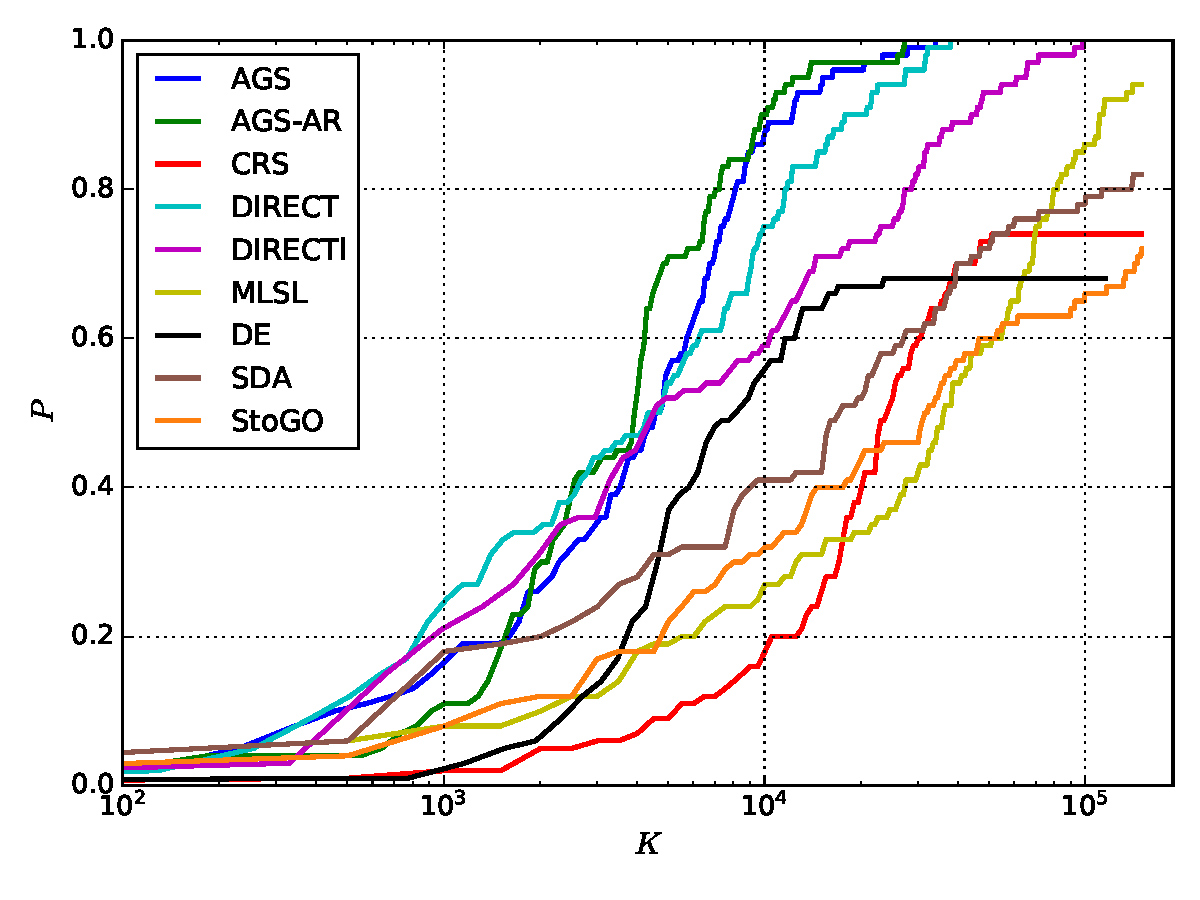
\includegraphics[width=.5\textwidth]{comparison/gklss4d.pdf}}\label{fig:s4d}}
    \subfloat[4d Hard]{{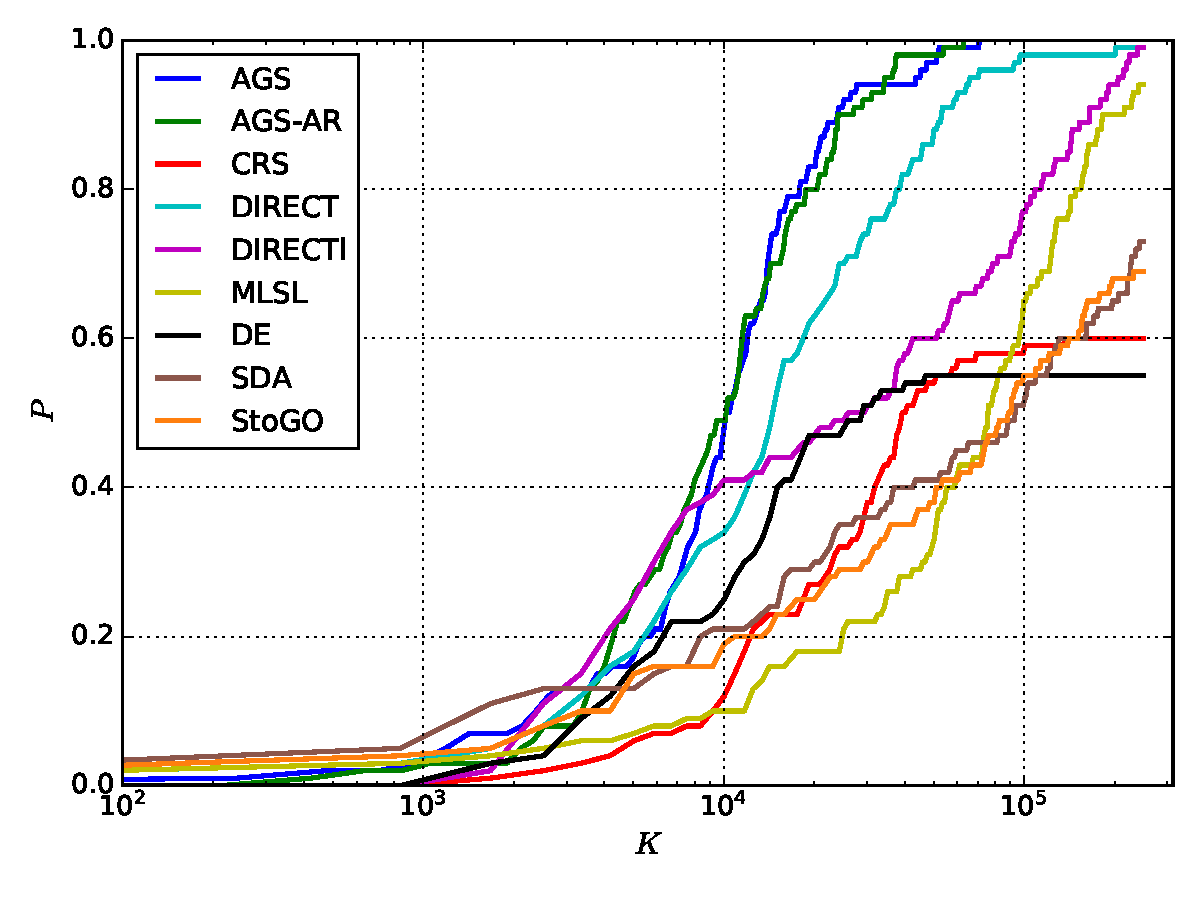
\includegraphics[width=.5\textwidth]{comparison/gklsh4d.pdf}}\label{fig:h4d}}
  \end{figure}
\end{frame}

\begin{frame}
  \frametitle{Результаты сравнения методов}
  \begin{figure}[ht]
    \centering
    \subfloat[5d Simple]{{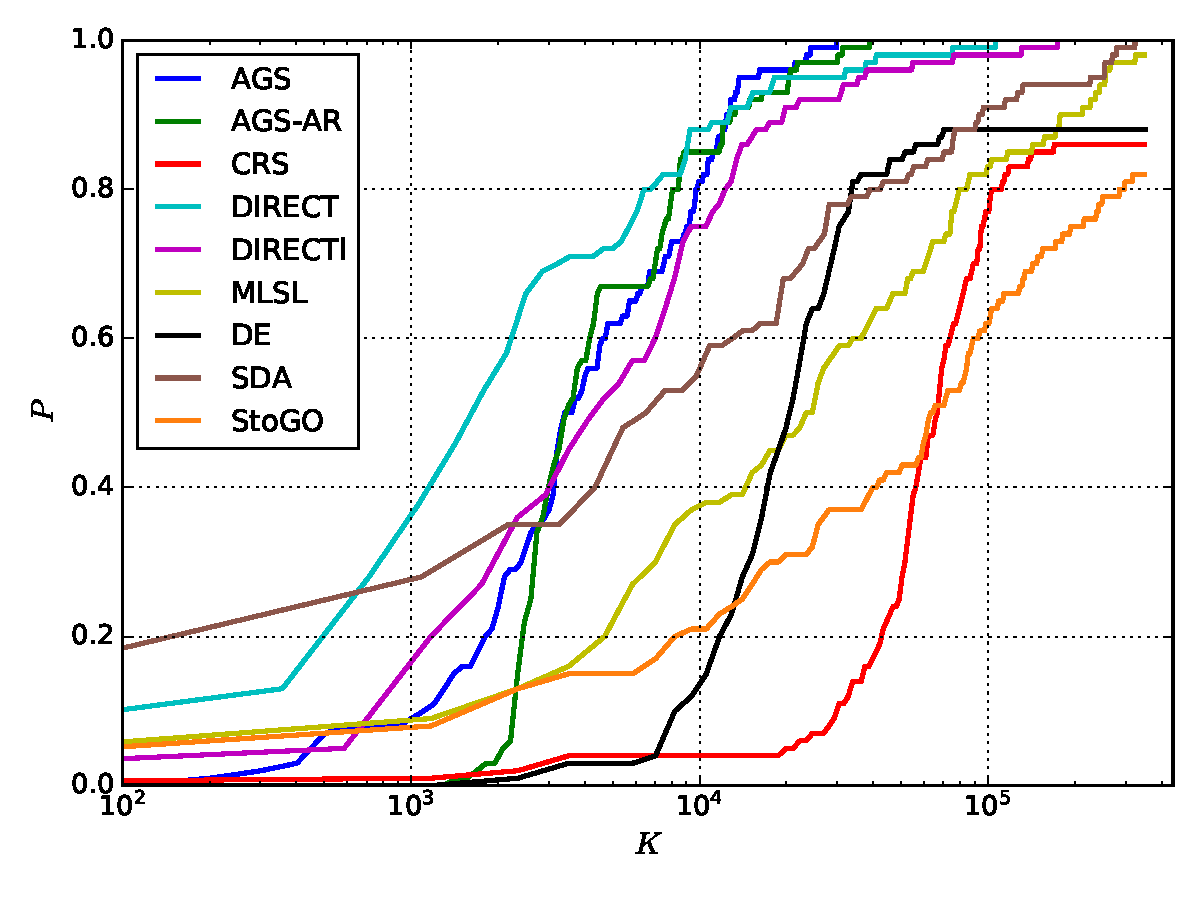
\includegraphics[width=.5\textwidth]{comparison/gklss5d.pdf}}\label{fig:s4d}}
    \subfloat[5d Hard]{{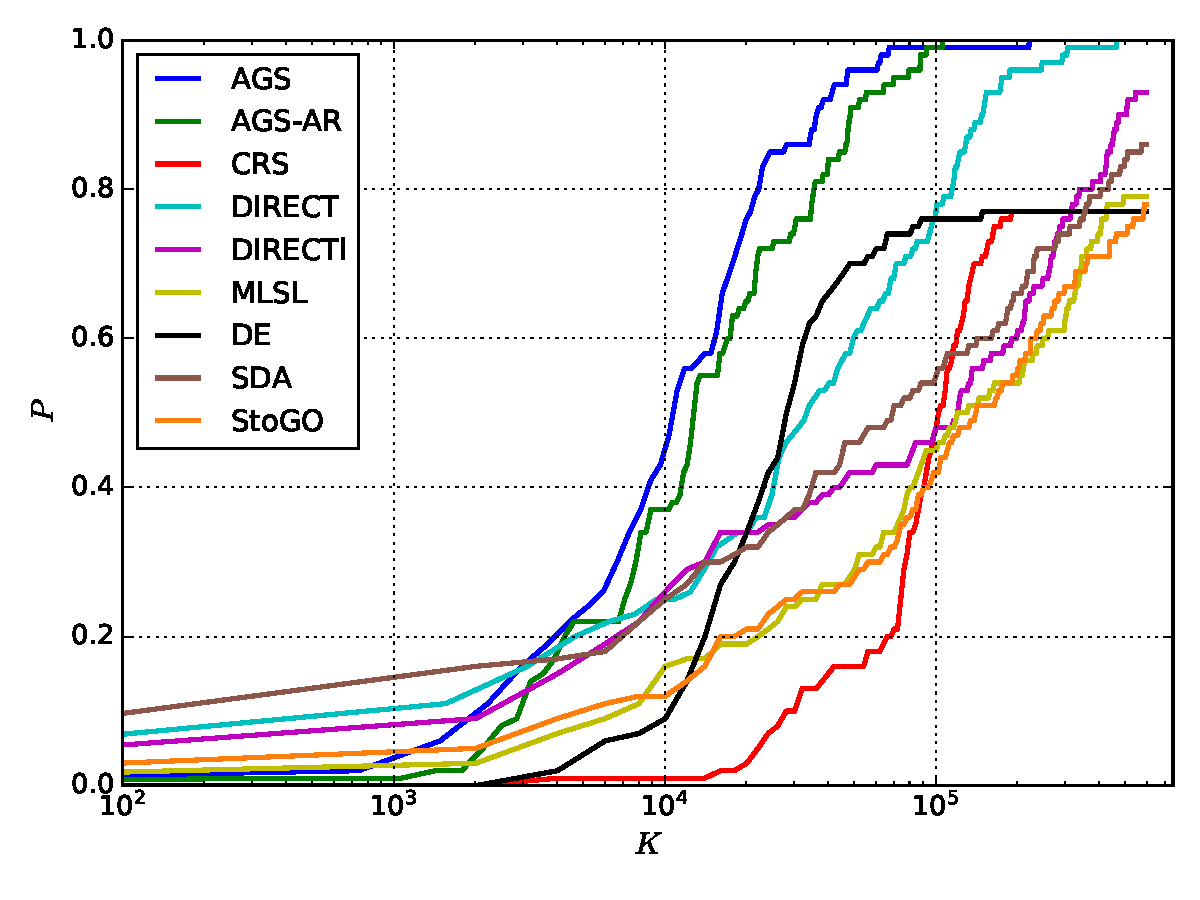
\includegraphics[width=.5\textwidth]{comparison/gklsh5d.pdf}}\label{fig:h4d}}
  \end{figure}
\end{frame}


\begin{frame}
  \frametitle{Метод, решающий множество задач}
  Метод опирается на ранее упомянутый алгоритм AGS (BarkalovK., StronginR., 2018):
  \begin{itemize}
    \item Создать \(q\) копий AGS, каждая из которых получает по одной задаче.
    \item Запустить \(q\) синхронно работающих копий AGS, но вместо выполнения Шага 3,
    остановить все копии и выбрать интервал с наибольшей характеристикой среди интервалов во всех задачах.
    \item Если выбранный на предыдущем шаге интервал принадлежит задаче \(i\), выполнить Шаг 3 в \(i^{th}\) копии AGS.
    Остальные копии пропускают Шаг 3.
    \item Чтобы обеспечить параллельность вычислений, метод выбирает \(p\) интервалов на предыдущих
    двух шагах и выполняет \(p\) испытаний параллельно.
  \end{itemize}
  Описанных алгоритм предполагает \textbf{сравнимость характеристик во всех задачах}.
\end{frame}

\begin{frame}
  \frametitle{Индексная схема учёта ограничений}
  Вместо исходной задачи с функциональными ограничениями, индексная схема рассматривает следующую задачу без ограничений:
  \begin{displaymath}
    \begin{array}{lr}
      \psi (x^{*})=\min_{x\in [0;1]}\psi (x), \\
      \psi (x)={\begin{cases}g_{\nu }(x)/H_{\nu }&\nu <M\\(g_{M}(x)-g_{M}^{*})/H_{M}&\nu =M\end{cases}},
    \end{array}
  \end{displaymath}
  где при \(\nu=m+1\;,g_\nu(x)=\varphi(x)\).

  Характеристики алгоритма глобального поиска при использовании индексной схемы (IAGS) имеют следующий вид:
  \begin{displaymath}
    R(i)={\begin{cases}\Delta _{i}+{\frac {(z_{i}-z_{i-1})^{2}}{(r_{\nu }\mu _{\nu })^{2}\Delta _{i}}}-2{\frac {z_{i}+z_{i-1}-2z_{\nu }^{*}}{r_{\nu }\mu _{\nu }}}&\nu =\nu (x_{i})=\nu (x_{i-1})\\2\Delta _{i}-4{\frac {z_{i-1}-z_{\nu }^{*}}{r_{\nu }\mu _{\nu }}}&\nu =\nu (x_{i-1})>\nu (x_{i})\\2\Delta _{i}-4{\frac {z_{i}-z_{\nu }^{*}}{r_{\nu }\mu _{\nu }}}&\nu =\nu (x_{i})>\nu (x_{i-1})\end{cases}}
  \end{displaymath}
  где \(z_i=\psi(x_i)\).

  \textit{\footnotesize	{Подробное описание индексной схемы приведено в Strongin R.G., Sergeyev Ya.D.: Global optimization with non-convex constraints. Sequential and parallel algorithms (2000), Chapter 7}}
\end{frame}

\begin{frame}
  \frametitle{Сходимость}
  \textbf{Достаточные условия сходимости AGS (Д. Л. Маркин, Р. Г. Стронгин, 1987)}:
  \begin{enumerate}
    \item \(G\ne\emptyset\), исходная задача имеет решение.
    \item Функции \(g_j(y)\leqslant 0, 1\leqslant j\leqslant m + 1\), липшицевы с
      константами \(L_i\) в гиперинтервале \(D\) (здесь \(g_{m+1}(y)=\varphi(y)\)).
    \item Начиная с некоторого момента значения оценок констант Гёльдара \(Н_i\) становятся достаточно большими.
  \end{enumerate}

  \textbf{Достаточные условия сходимости MIAGS}: пусть указанные выше условия выполнены для
  каждой задачи \(i,\:1\leqslant i\leqslant q\) из (\ref{eq:many_problems}),
  т.е. каждая из задач может быть решена AGS.
    Тогда в процессе решения \(q\) задач MIAGS сгенерирует
    \(q\) бесконечных последовательностей \(\{y^k_i\},\:1\leqslant i\leqslant q\), таких, что
    \begin{displaymath}
      \varphi_i(\overline{y_i})=\inf\{ \varphi(y^k_i): g^i_j(y^k_i)\leqslant 0,1\leqslant j\leqslant m_i, k=1,2,\dots\}=\varphi_i(y^*_i).
    \end{displaymath}
\end{frame}

\begin{frame}
  \frametitle{Пример решения многокритериальной задачи}
  Рассмотрим следующую задачу:
  \begin{displaymath}
    \begin{array}{l}
        Minimize \left \{
        \begin{array}{l}
          f_1(y) = 4 y_1^2 + 4 y_2^2 \\
          f_2(y) = (y_1-5)^2 + (y_2-5)^2 \\
        \end{array}
        \right .
        y_1\in [-1;2],y_2\in [-2;1]
        \\s.t.
        \\
        \left \{
        \begin{array}{l}
          g_1(y) = (y_1 - 5)^2 + y_2^2 - 25 \leqslant 0 \\
          g_2(y) = -(y_1 - 8)^2 - (y_2 + 3)^2 + 7.7 \leqslant 0\\
        \end{array}
        \right .
    \end{array}
  \end{displaymath}
  После скаляризации задача примет следующую форму:
  \begin{displaymath}
    \varphi(y^*(\lambda_1,\lambda_2))=\min_{y\in D}\max\{\lambda_1 f_1(y), \lambda_2 f_2(y)\};\lambda_1,\lambda_2\in[0,1],\: \lambda_1+\lambda_2=1
\end{displaymath}
Для численного постороения Парето фронта рассмотрим
100 пар \((\lambda_1,\lambda_2)\) таких, что
\(\lambda_1^i=i h,\: \lambda_2^i=1-\lambda_1^i,\: h=10^{-2},i=\overline{1, 100}\).
\end{frame}

\begin{frame}
  \frametitle{Пример решения многокритериальной задачи}
  \vspace*{-1.0cm}
  \begin{displaymath}
    \begin{array}{cr}\\
      SP(S)=\sqrt{\frac{1}{|S|-1} \sum_{i=1}^{|S|} (\overline{d}-d_i)^2},\:\overline{d}=mean\{d_i\}, \\
      d_i=\min_{s_i,s_j\in S:s_i\ne s_j}||F(s_i)-F(s_j)||_1,\: F=(f_1,f_2)
    \end{array}
  \end{displaymath}

  \begin{figure}[ht]
      \centering
      \vspace*{-0.5cm}
      \subfloat[IAGS, \(SP_{single}=0.984\)]{
      \label{fig:mco_pareto_1} {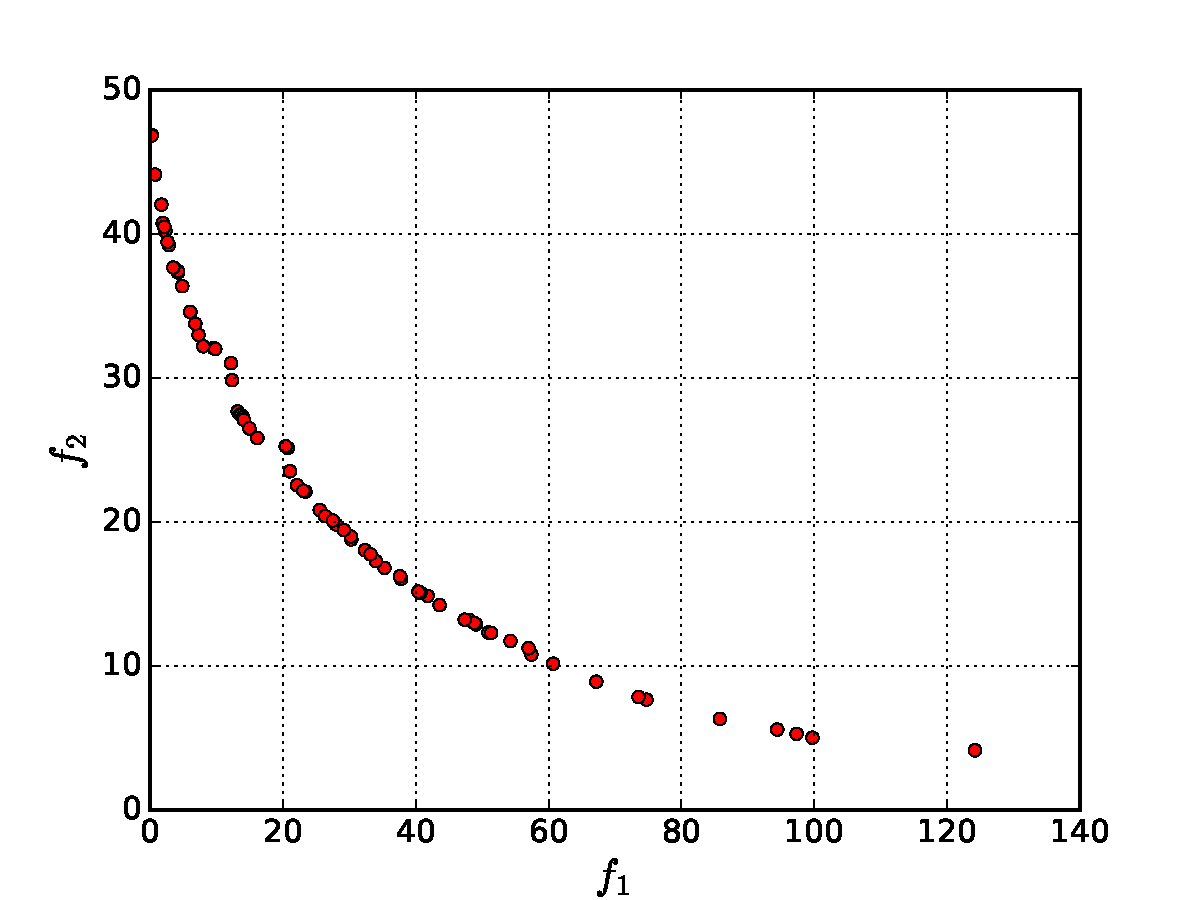
\includegraphics[width=.5\textwidth]{single_mco.pdf}}}
      \subfloat[MIAGS, \(SP_{multi}=0.749\)]{
      \label{fig:mco_pareto_2} {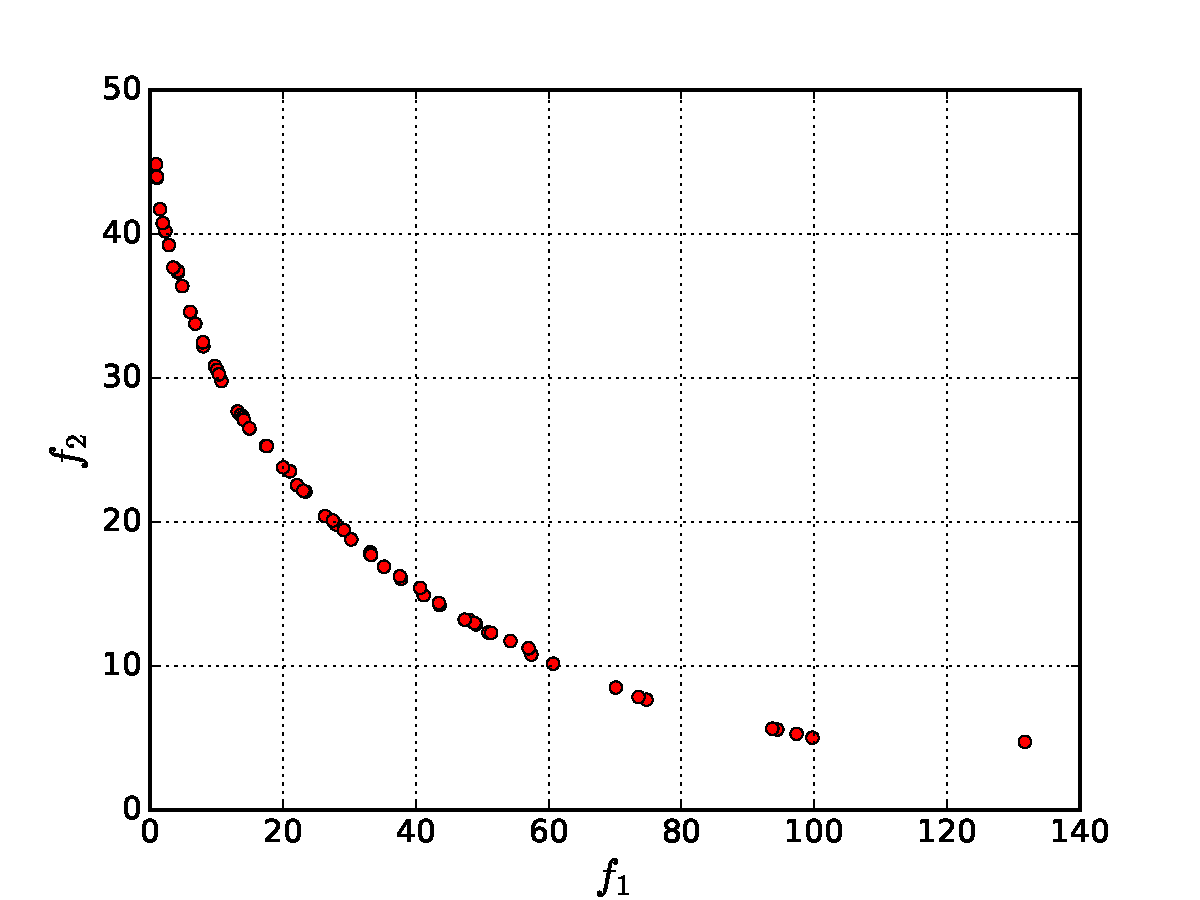
\includegraphics[width=.5\textwidth]{multi_mco.pdf}}}
      \caption{Численные оценки множества Парето, полученные после 2500 испытаний}
      \label{fig:mco_pareto}
  \end{figure}
\end{frame}

\begin{frame}
  \frametitle{Решение тестовых задач с ограничениями}
  \begin{columns}
    \begin{column}{0.5\textwidth}
      Наборы задач с ограничениями были получены путём применения системы
      GCGen к функциям, порождёнными генераторами задач без ограничений.
      Основные свойства полученных наборов задач:
      \begin{itemize}
        \item \(q\)=100;
        \item Размерность 2, 3 или 4;
        \item Базовые функции GKLS или \(F_{GR}\), или их комбинация;
        \item Количество нелинейных ограничений: 2.
      \end{itemize}
    \end{column}
    \begin{column}{0.5\textwidth}
      \centerline{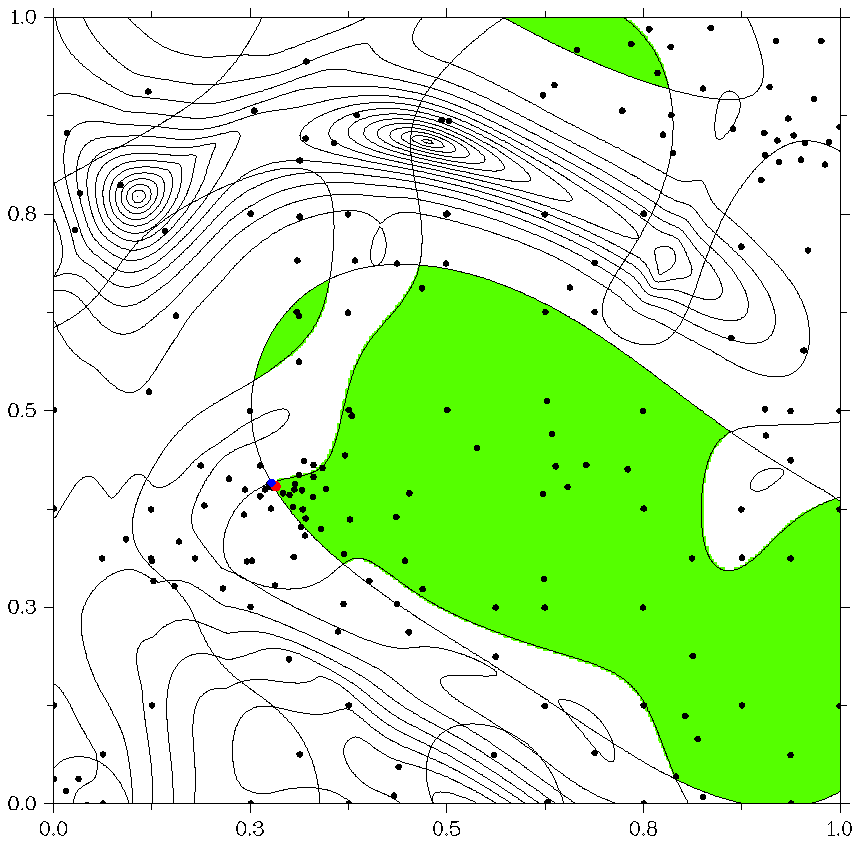
\includegraphics[width=0.9\textwidth]{4.png}}
    \end{column}
  \end{columns}
  \footnotesize{GCGen is available here: \textit{https://github.com/UNN-ITMM-Software/GCGen}}
\end{frame}

\begin{frame}
  \frametitle{Аппаратное и программное окружение}
  \begin{center}
    Параллельный метод реализован на языке C++ с использованием технологии OpenMP
    для параллельных вычислений на общей памяти.

    Все численные эксперименты были выполнены на машине со следующей конфигурацией:
    Intel Core i7-7800X (6 cores) CPU, 64GB RAM, Unubtu 16.04 ОS, GCC 5.5 compiler.
    
    В целевые функции и ограничения во всех задачах вносились задержки так, чтобы
    вычисление каждой функции занимало 1 мс.
  \end{center}
\end{frame}

\begin{frame}
  \frametitle{Результаты решения тестовых задач}
  \begin{figure}[ht]
    \vspace*{-0.5cm}
      \centering
      \subfloat[\(D_{max}\)]{
      \label{fig:max_dev} {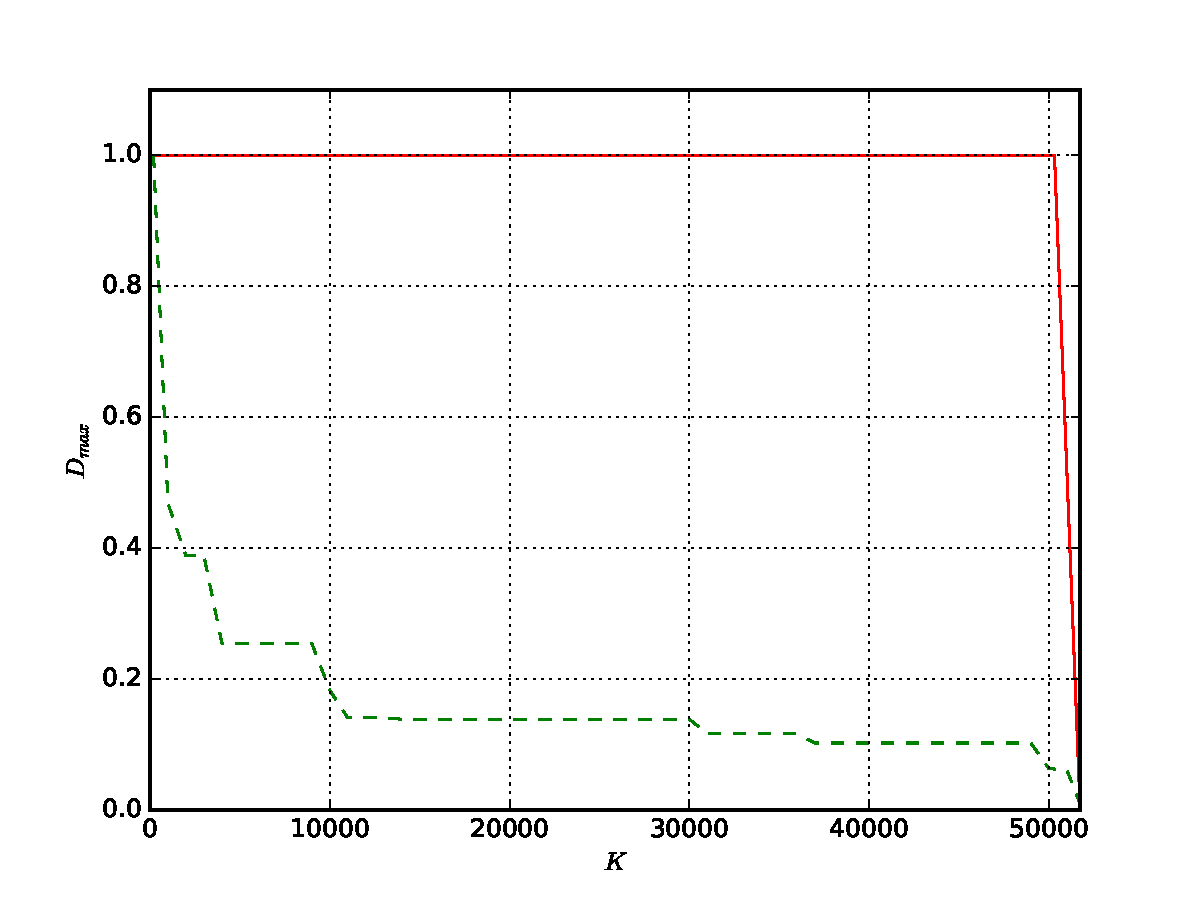
\includegraphics[width=.5\textwidth]{mixed_2d_max.pdf}}}
      \subfloat[\(D_{avg}\)]{
      \label{fig:avg_dev} {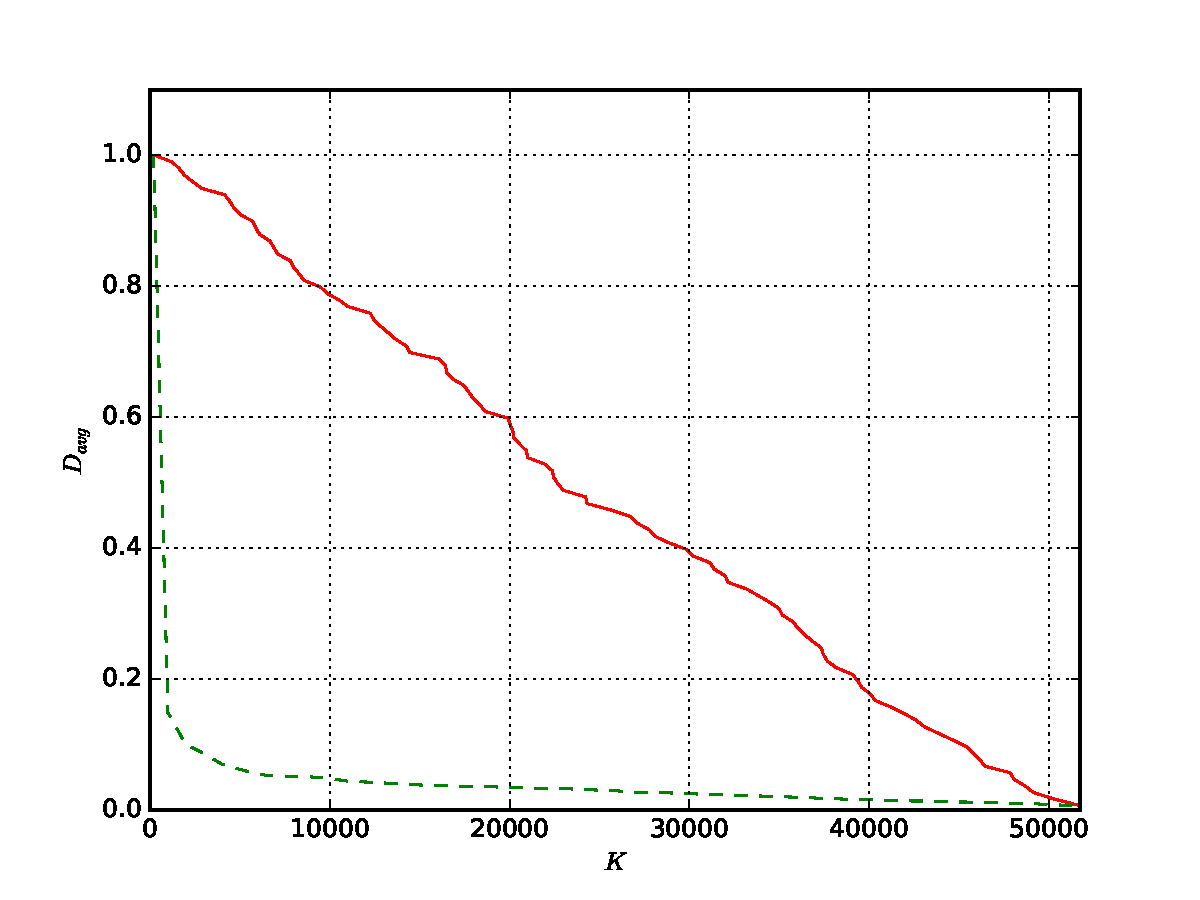
\includegraphics[width=.5\textwidth]{mixed_2d_avg.pdf}}}
      \caption{Изменение средней и максимальной ошибки, при решении смешанного класса задач, 
      полученного с помощью двух генераторов: GKLS и \(F_{GR}\)}
      \label{fig:devs_mixed}
  \end{figure}
\end{frame}

\begin{frame}
  \frametitle{Результаты решения тестовых задач}
  \begin{table}
    \centering
    \begin{tabular}{c|c|c|c|c|c}
      %\cline{1-8}\noalign{\smallskip}
      Класс задач & \textit{p} & Количество итераций & Время, с & \(S_i\) & \(S_t\)   \\
      %s\noalign{\smallskip} \cline{4-5} \cline{7-8}  \noalign{\smallskip}
      \hline
      GKLS \& \(F_{GR}\)-based \
        & 1 & 51434 & 90.20 & -    & - \\
        & 2 & 25698 & 56.96 & 2.00 & 1.58 \\
        & 4 & 13015 & 36.67 & 3.95 & 2.46 \\
        & 6 & 8332  & 26.85 & 6.17 & 3.36 \\
      \hline
      GKLS-based 2d \
        & 1 & 59066 & 97.53 & -    & - \\
        & 2 & 29060 & 60.56 & 2.04 & 1.61 \\
        & 4 & 14266 & 38.92 & 4.14 & 2.51 \\
        & 6 & 9436  & 29.53 & 6.26 & 3.30 \\
      \hline
    \end{tabular}
  \end{table}
\end{frame}
\begin{frame}
  \frametitle{Результаты решения тестовых задач}
  \begin{table}
    \centering
    \begin{tabular}{c|c|c|c|c|c}
      %\cline{1-8}\noalign{\smallskip}
      Класс задач & \textit{p} & Количество итераций & Время, с & \(S_i\) & \(S_t\)   \\
      %s\noalign{\smallskip} \cline{4-5} \cline{7-8}  \noalign{\smallskip}
      \hline
      GKLS-based 3d \
        & 1 & 782544 & 1117.55 & -    & - \\
        & 2 & 397565 & 752.92  & 1.97 & 1.48 \\
        & 4 & 208073 & 526.67  & 3.76 & 2.12 \\
        & 6 & 142089 & 445.45  & 5.50 & 2.51 \\
      \hline
      GKLS-based 4d \
        & 1 & 14021720 & 15806.6 & -    & - \\
        & 2 & 6313070 & 7254.85  & 2.22 & 2.18 \\
        & 4 & 3479344 & 4932.55  & 4.03 & 3.20 \\
        & 6 & 2783339 & 3955.38  & 5.04 & 3.99 \\
      \hline
    \end{tabular}
  \end{table}
\end{frame}
\begin{frame}
  \frametitle{Заключение}
  В ходе выполнения работы были получены следующие результаты:
  \begin{enumerate}
      \item Произведено сравнение различных способов редукции размерности, основанных на отображениях типа кривой Пеано;
      \item Предложена модификация AGS, AGS-AR, менее чувствительная к параметрам; AGS-AR продемонстрировал надёжность и скорость
      сходимости на уровне другого детерминированного метода, DIRECT,
      и превзошёл на рассмотренных тестовых задачах многие другие методы, реализации которых так же доступны в исходных кодах.
      Программная реализация метода AGS-AR прошла процедуру ревью и была включена в состав популярной библиотеки
      алгоритмов нелинейной оптимизации NLOpt;
      \item Реализована поддержка нелинейных ограничений в алгоритме, решающeм
      множество задач глобальной оптимизации в совокупности и распределяющего свои ресурсы так, чтобы
      обеспечивать равномерную сходимость во всех задачах. Доказано теорема о достаточных условиях сходимости
      полученного метода. Свойство равномерной сходимости проверено с помощью численного эксперимента.
  \end{enumerate}
\end{frame}

{
\unnumbered
\begin{frame}{{}}
  \frametitle{Q\&A}
  \begin{center}
    %\Large{Контакты:}
\vspace{0.5cm}

    sovrasov.vladislav@itmm.unn.ru

    https://github.com/sovrasov
  \end{center}
\end{frame}
}
\end{document}
